\chapter{Codice CFD}

Una volta realizzata la mesh, come descritto nel capitolo precedente, il file
\texttt{.msh} generato da Gmsh viene passato al codice CFD.
Il codice risolve le equazioni di Eulero 2D (di cui si trovano i fondamenti
nel capitolo teorico) ed è scritto in Fortran~90 per le sue alte prestazioni
nel calcolo numerico.
L'architettura è modulare: un modulo di strutture dati
(\texttt{strutture.f90}), un modulo di variabili globali
(\texttt{Variabili.f90}), un programma principale (\texttt{main.f90}) e
una serie di subroutine specializzate, ognuna responsabile di una fase
precisa del ciclo di soluzione.

% ============================================================
\section{Modulo \texttt{strutture.f90}}
% ============================================================

\begin{figure}[H]
    \centering
    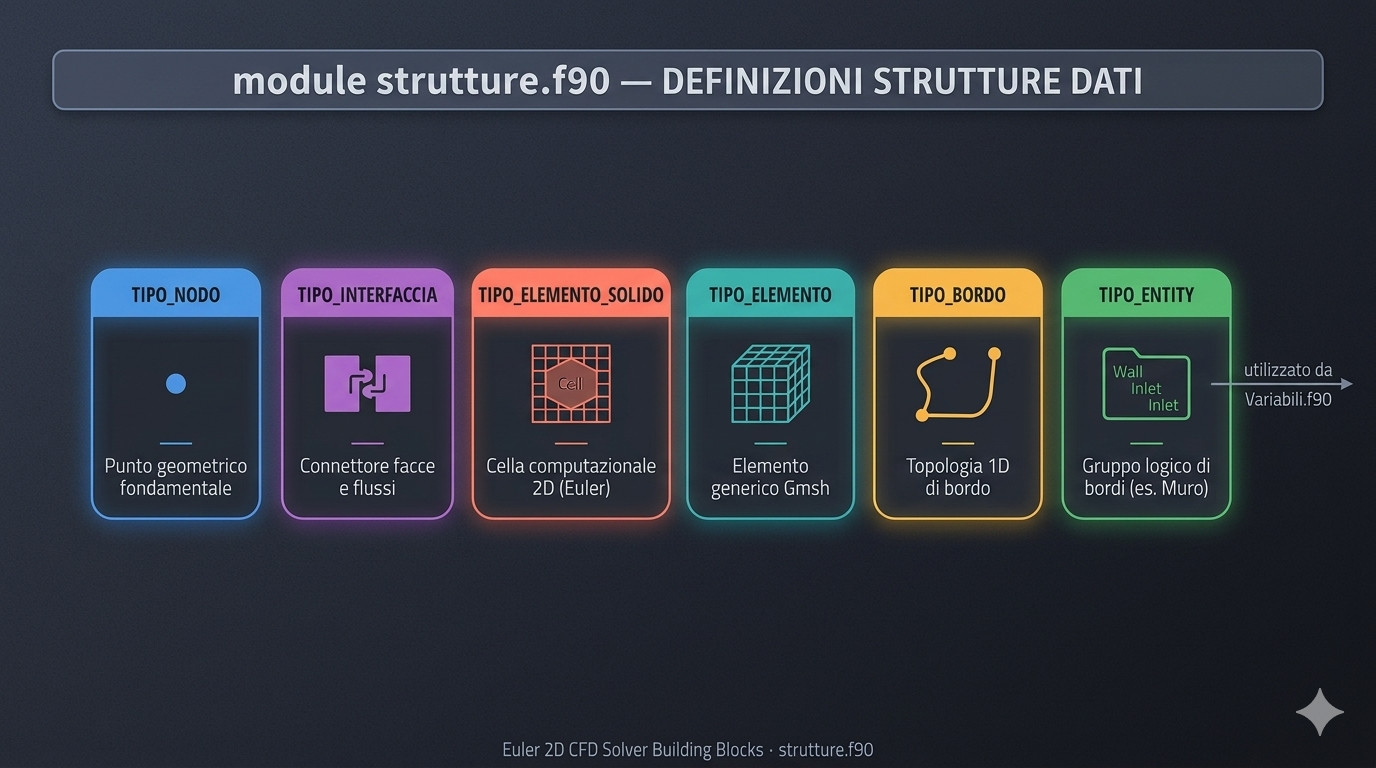
\includegraphics[width=0.88\textwidth]{../Images/strutture.png}
    \caption{Rappresentazione grafica delle sei strutture dati definite in
    \texttt{strutture.f90}: \texttt{TIPO\_NODO}, \texttt{TIPO\_INTERFACCIA},
    \texttt{TIPO\_ELEMENTO\_SOLIDO}, \texttt{TIPO\_ELEMENTO},
    \texttt{TIPO\_BORDO}, \texttt{TIPO\_ENTITY}.}
    \label{fig:strutture}
\end{figure}

Il modulo \texttt{strutture.f90} definisce i tipi derivati (strutture) che
consentono di organizzare in modo compatto tutti i dati geometrici e fisici
letti dal file di Gmsh.
Le strutture sono sei, ognuna con un ruolo preciso nella rappresentazione
della mesh e del campo di moto.

\subsection{\texttt{tipo\_elemento}}

Rappresenta un elemento generico letto dal file \texttt{.msh} di Gmsh,
prima che venga classificato come cella interna o di bordo.
Contiene il numero di nodi, il tipo di elemento nel formato Gmsh
(es.\ triangolo, quadrilatero), l'array dei tag dei nodi associati e il
tag di entity.

\begin{lstlisting}[style=fortran]
type tipo_elemento
    integer :: nnodi, tipo_ele   ! tipo_ele: tag gmsh dell'elemento
    integer, dimension(:), pointer :: nodi
    integer :: entity
end type tipo_elemento
\end{lstlisting}

\subsection{\texttt{tipo\_nodo}}

Rappresenta un punto geometrico della mesh con le sue coordinate e
le informazioni di connettività topologica.
\texttt{nghbr} contiene i tag dei nodi vicini; \texttt{ele} contiene i tag
degli elementi che condividono quel nodo.

\begin{lstlisting}[style=fortran]
type tipo_nodo
    real(4), dimension(2) :: x       ! coordinate (x, y)
    integer :: nnghbrs, neles
    integer, dimension(:), allocatable :: nghbr
    integer, dimension(:), allocatable :: ele
end type tipo_nodo
\end{lstlisting}

\subsection{\texttt{tipo\_interfaccia}}

Rappresenta un'interfaccia tra due celle computazionali (o tra una cella
e un bordo) ed è il luogo dove vengono calcolati i flussi numerici.
La convenzione è che \texttt{e1} è l'elemento di riferimento per la
normale uscente.

\begin{lstlisting}[style=fortran]
type tipo_interfaccia
    integer :: e1, e2              ! celle ai lati dell'interfaccia
    integer :: edge_e1, edge_e2    ! indici dei lati corrispondenti
    integer :: nodo1, nodo2        ! nodi agli estremi
    real(4), dimension(2) :: normal, x0  ! normale uscente, baricentro
    real(4) :: length              ! lunghezza dell'interfaccia
    integer :: entity
    real(4), dimension(4) :: f     ! flussi (4 componenti Eulero 2D)
    integer :: int_perio           ! 10=interno, altro=bordo periodico
end type tipo_interfaccia
\end{lstlisting}

\subsection{\texttt{tipo\_elemento\_solido}}

È la struttura principale del solutore: rappresenta una cella
computazionale 2D interna su cui viene risolta l'equazione di Eulero.
Contiene sia le proprietà geometriche (area, baricentro, connettività)
sia le variabili fisiche (conservative e primitive) e le derivate
temporali.

\begin{lstlisting}[style=fortran]
type tipo_elemento_solido
    integer :: nnodi, tipo_ele, nlati
    integer, dimension(:), allocatable :: nodi
    integer, dimension(:,:), allocatable :: edge
    integer :: nnghbrs
    integer, dimension(:), allocatable :: nghbr
    integer, dimension(:), allocatable :: interfaces
    real(4) :: area
    real(4), dimension(2) :: x0
    real(4), dimension(4) :: ucons   ! variabili conservative
    real(4) :: u, v, a, P, T, S      ! variabili primitive
    real(4), dimension(4) :: d_dt    ! derivate temporali
end type tipo_elemento_solido
\end{lstlisting}

Il vettore \texttt{ucons} contiene le quattro variabili conservative:
\[
\mathtt{ucons} =
\begin{Bmatrix} \rho E \\ \rho \\ \rho u \\ \rho v \end{Bmatrix}
\]
Il vettore \texttt{d\_dt} ne contiene le derivate temporali, accumulate
durante il calcolo dei flussi e usate per l'aggiornamento esplicito:
\[
\mathtt{d\_dt} =
\begin{Bmatrix}
  \partial(\rho E)/\partial t \\
  \partial\rho/\partial t \\
  \partial(\rho u)/\partial t \\
  \partial(\rho v)/\partial t
\end{Bmatrix}
\]

\subsection{\texttt{tipo\_bordo} e \texttt{tipo\_entity}}

\texttt{tipo\_bordo} rappresenta la topologia 1D di un bordo del dominio
(sequenza di interfacce al contorno).
\texttt{tipo\_entity} è un gruppo logico di bordi (es.\ \texttt{Wall},
\texttt{Inlet}, \texttt{Outlet}) ed è utilizzato dal modulo
\texttt{Variabili.f90} per gestire le condizioni al contorno.

% ============================================================
\section{Modulo \texttt{Variabili.f90}}
% ============================================================

\begin{figure}[H]
    \centering
    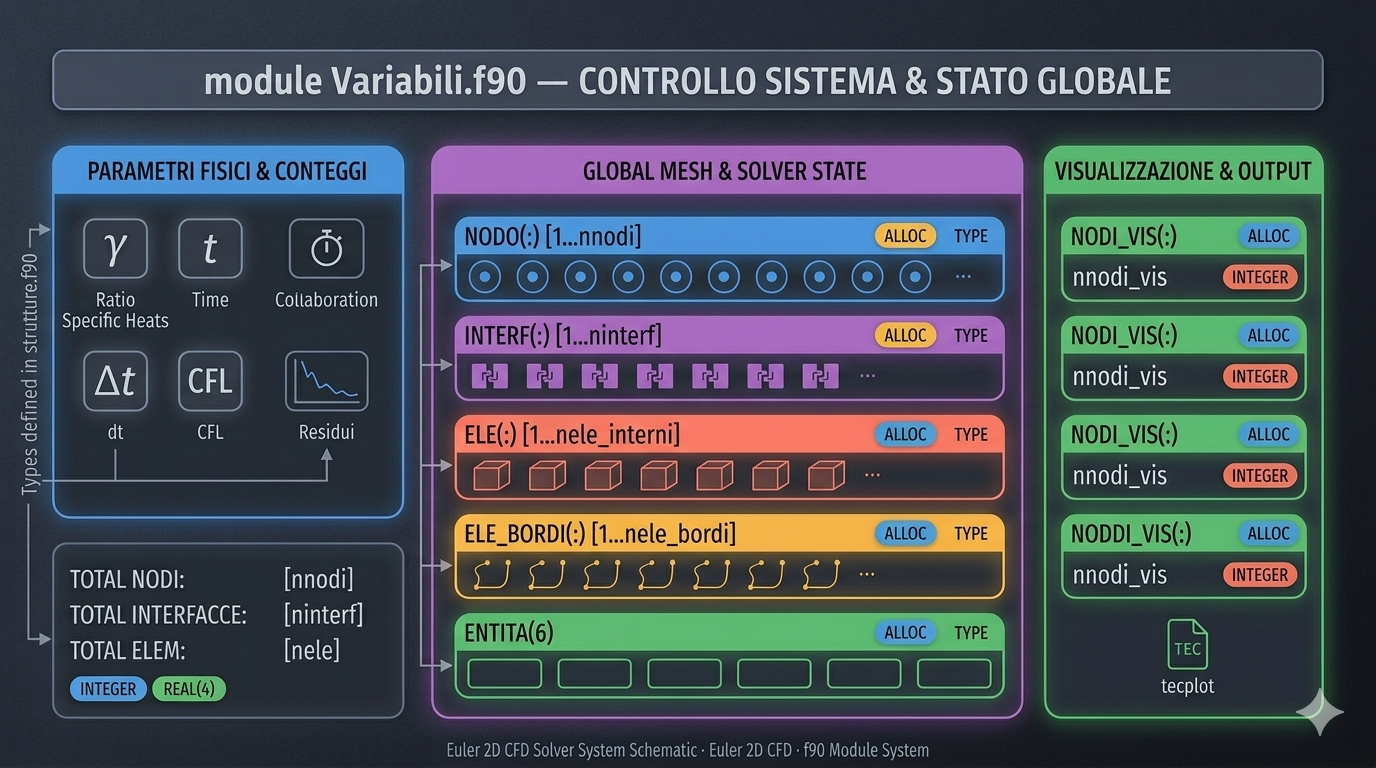
\includegraphics[width=0.88\textwidth]{../Images/variabili.png}
    \caption{Schema del modulo \texttt{Variabili.f90}: parametri fisici e
    conteggi (sinistra), stato globale della mesh e del solutore (centro),
    strutture per la visualizzazione e output Tecplot (destra).}
    \label{fig:variabili}
\end{figure}

Il modulo \texttt{Variabili.f90} funge da stato globale del programma:
importa i tipi da \texttt{strutture.f90} e dichiara tutte le variabili
allocabili che vengono condivise tra le varie subroutine tramite la
clausola \texttt{use Variabili}.

\begin{lstlisting}[style=fortran]
Module Variabili
    use strutture
    implicit none
    save

    ! Contatori del ciclo temporale
    integer :: k, kinf, kout, kfinal

    ! Parametri fisici e coefficienti adimensionali
    real(4) :: gam, GA, GB, GC, GD, GE, GF, GG, GH, GI, GJ

    ! Controllo temporale
    real(4) :: time, dt, CFL, periodo

    ! Nome file mesh
    character(100) :: mesh_file

    ! Condizioni al contorno
    real(4) :: ttotin, ptotin, alpha, pexit, machin

    ! Dimensioni della mesh
    integer :: nnodi, ninterf, nele, nele_interni, nele_bordi
    integer :: nentity, ndim, neqs

    ! Residui
    real(4), dimension(4) :: norm2_residuals, norminf_residuals

    ! Array allocabili della mesh (tipi da strutture.f90)
    type(tipo_nodo),           dimension(:), allocatable :: nodo
    type(tipo_interfaccia),    dimension(:), allocatable :: interf
    type(tipo_elemento),       dimension(:), allocatable :: ele_all
    type(tipo_elemento_solido),dimension(:), allocatable :: ele
    type(tipo_bordo),          dimension(:), allocatable :: ele_bordi
    type(tipo_entity)                                    :: entita(6)
End Module
\end{lstlisting}

I contatori \texttt{kinf} e \texttt{kout} controllano rispettivamente la
frequenza di stampa dei residui a schermo e la frequenza di scrittura dei
file Tecplot \texttt{.plt}.
I coefficienti \texttt{GA}--\texttt{GJ} sono combinazioni di $\gamma$
precalcolate per efficienza (es.\ $GA = \gamma - 1$, $GB = \gamma/(\gamma-1)$,
ecc.).

% ============================================================
\section{Programma Principale \texttt{main.f90}}
% ============================================================

Il programma principale orchestra il ciclo di soluzione richiamando le
subroutine nell'ordine corretto: lettura dati, costruzione della mesh,
inizializzazione del campo, ciclo temporale.

\begin{lstlisting}[style=fortran]
Program test2d
    use Variabili
    implicit none

    ! Pulizia file di output precedenti
    call system("del *.plt")   ! Windows
    ! call system("rm *.plt")  ! Linux

    call input              ! lettura parametri e condizioni al contorno
    call leggi_gmsh         ! parsing del file .msh e costruzione mesh
    call processa_elementi  ! calcolo geometria (aree, normali, baricentri)
    call init               ! inizializzazione campo di moto

    call write_tecplot_file(0, 0.)
    time = 0.

    do k = 1, kfinal
        call compute_dt       ! calcolo passo temporale CFL
        call compute_fluxes   ! calcolo flussi alle interfacce + d_dt
        call integ_time       ! aggiornamento variabili conservative

        time = time + dt

        if (mod(k, kinf) == 0) then
            write(*,*) 'k, time, dt = ', k, time, dt
            call compute_norm_residuals
        end if

        if (mod(k, kout) == 0) then
            call write_tecplot_file(k, 0.)
        end if
    end do
End Program
\end{lstlisting}

% ============================================================
\section{Subroutine \texttt{input}}
% ============================================================

Gestisce la lettura dei tre file di configurazione della simulazione:
\begin{itemize}
    \item \texttt{input.txt}: nome del file mesh, \texttt{KFINAL}
          (numero di iterazioni), \texttt{KINF} (frequenza residui),
          \texttt{KOUT} (frequenza output), \texttt{CFL}.
    \item \texttt{inlet.txt}: $T^\circ_{\rm in}$, $P^\circ_{\rm in}$,
          $\alpha$ (angolo del flusso), $M_{\rm in}$.
    \item \texttt{outlet.txt}: pressione statica di uscita $P_{\rm exit}$.
\end{itemize}
I valori letti vengono salvati nelle variabili globali del modulo
\texttt{Variabili}.

% ============================================================
\section{Subroutine \texttt{leggi\_gmsh}}
% ============================================================

Apre e analizza il file \texttt{.msh} prodotto da Gmsh.
La subroutine esegue i seguenti passi:
\begin{enumerate}
    \item Legge il blocco \texttt{\$Nodes} e alloca l'array \texttt{nodo(:)},
          popolando le coordinate di ogni nodo.
    \item Legge il blocco \texttt{\$Elements} e alloca \texttt{ele\_all(:)},
          distinguendo gli elementi in base al tipo Gmsh (triangoli e
          quadrilateri sono celle interne; linee sono elementi di bordo).
    \item Separa gli elementi interni in \texttt{ele(:)} (tipo
          \texttt{tipo\_elemento\_solido}) e gli elementi di bordo in
          \texttt{ele\_bordi(:)}.
    \item Costruisce le interfacce \texttt{interf(:)} identificando i lati
          condivisi tra celle adiacenti e i lati di bordo.
    \item Popola le strutture \texttt{entita(:)} raggruppando i bordi per
          tag di entity (parete, inlet, outlet, ecc.).
\end{enumerate}

% ============================================================
\section{Subroutine \texttt{processa\_elementi}}
% ============================================================

Calcola le proprietà geometriche di celle e interfacce a partire dalla
connettività nodale.

\paragraph{Baricentro.}
Calcolato come media aritmetica delle coordinate dei nodi dell'elemento:
\[
  \bm{x}_0 = \frac{1}{N_{\rm nodi}} \sum_{k=1}^{N_{\rm nodi}} \bm{x}_k
\]

\paragraph{Area.}
Calcolata tramite la formula di Erone a partire dalle lunghezze dei lati
$a$, $b$, $c$ e del semiperimetro $p = (a+b+c)/2$:
\[
  A = \sqrt{p\,(p-a)(p-b)(p-c)}
\]

\paragraph{Normale e lunghezza delle interfacce.}
Per ogni interfaccia delimitata dai nodi $\bm{x}_1$ e $\bm{x}_2$:
\begin{itemize}
    \item la lunghezza è $l = \|\bm{x}_2 - \bm{x}_1\|$;
    \item il versore tangente è $\hat{t} = (\bm{x}_2 - \bm{x}_1)/l$;
    \item il versore normale uscente da \texttt{e1} è
          $\hat{n} = (t_y,\,-t_x)$ (rotazione di $90°$ di $\hat{t}$,
          orientata in modo che punti verso l'esterno di \texttt{e1}).
\end{itemize}

% ============================================================
\section{Subroutine \texttt{init}}
% ============================================================

Inizializza il campo di moto su tutte le celle computazionali a partire
dalle condizioni all'inlet, applicando le relazioni isentropiche.
Le variabili conservative \texttt{ucons} di ogni cella vengono impostate
al valore uniforme corrispondente alle condizioni di ingresso (flusso
uniforme iniziale); le variabili primitive ($u$, $v$, $a$, $P$, $T$, $S$)
vengono derivate di conseguenza.
Le variabili sono espresse in forma adimensionale rispetto alle grandezze
di riferimento $P^\circ_{\rm in}$ e $T^\circ_{\rm in}$, come descritto
nel capitolo teorico (Sezione~\ref{sec:adim}).

% ============================================================
\section{Subroutine \texttt{compute\_dt}}
% ============================================================

Calcola il passo temporale globale $\Delta t$ ad ogni iterazione
imponendo la condizione di stabilità CFL su tutte le celle:
\[
  \Delta t = \text{CFL} \cdot \min_{i=1,\ldots,N_{\rm ele}}
  \frac{\sqrt{A_i}}{|\bm{q}_i| + a_i}
\]
dove $A_i$ è l'area della cella $i$, $\bm{q}_i$ la velocità del fluido e
$a_i$ la velocità del suono locale.
Il minimo è preso su tutti gli elementi interni, garantendo che il passo
temporale soddisfi il criterio di stabilità nella cella più restrittiva.
Il valore risultante viene salvato nella variabile globale \texttt{dt}.

% ============================================================
\section{Subroutine \texttt{compute\_fluxes}}
% ============================================================

È la subroutine computazionalmente più onerosa: calcola i flussi numerici
$\Fvec_{ij}$ su tutte le interfacce e ne accumula il contributo nella
derivata temporale \texttt{d\_dt} di ogni cella, secondo la formula
ai volumi finiti (Eq.~\ref{eq:volumi_finiti} del capitolo teorico).

Per ogni interfaccia interna vengono eseguiti i seguenti passi:
\begin{enumerate}
    \item Recupero degli stati $L$ (cella \texttt{e1}) e $R$ (cella
          \texttt{e2}) in termini di variabili conservative.
    \item Rotazione degli stati nel sistema di riferimento locale
          dell'interfaccia (allineato con la normale $\hat{n}$).
    \item Calcolo del flusso numerico con lo schema scelto
          (Lax--Friedrichs o Roe), entrambi descritti nella
          Sezione~\ref{sec:flussi} del capitolo teorico.
    \item Rotazione inversa del flusso nel sistema globale.
    \item Aggiornamento di \texttt{d\_dt} per le celle \texttt{e1} e
          \texttt{e2} con segni opposti (normale uscente da \texttt{e1}
          è entrante in \texttt{e2}).
\end{enumerate}
Le interfacce di bordo vengono trattate separatamente, applicando le
condizioni al contorno appropriate (parete, inlet subsonico/supersonico,
outlet subsonico/supersonico).

% ============================================================
\section{Subroutine \texttt{integ\_time}}
% ============================================================

Aggiorna le variabili conservative di tutte le celle con lo schema di
Eulero esplicito in avanti, utilizzando le derivate temporali accumulate
da \texttt{compute\_fluxes}:
\[
  \mathtt{ucons}_i^{k+1} = \mathtt{ucons}_i^k + \Delta t \cdot \mathtt{d\_dt}_i^k
\]

\begin{lstlisting}[style=fortran]
subroutine integ_time
    use variabili
    implicit none
    integer :: i

    do i = 1, nele_interni
        ! Aggiornamento variabili conservative
        ele(i)%ucons(:) = ele(i)%ucons(:) + dt * ele(i)%d_dt(:)

        ! Ricalcolo variabili primitive dalle conservative
        ele(i)%u = ele(i)%ucons(3) / ele(i)%ucons(2)
        ele(i)%v = ele(i)%ucons(4) / ele(i)%ucons(2)
        ! ... pressione, temperatura, velocita' del suono, entropia
    end do
end subroutine
\end{lstlisting}

Dopo l'aggiornamento delle variabili conservative, le variabili primitive
($u$, $v$, $P$, $T$, $a$, $S$) vengono ricalcolate per essere disponibili
al passo successivo nella subroutine \texttt{compute\_fluxes} e per
l'output.
